O modelo foi implementado na linguagem Julia\footnote{Site oficial da linguagem:
\url{https://julialang.org/}.}. Como discutido na página oficial da linguagem, o
design da linguagem é pensado tendo em vista a computação científica, buscando
tanto performance quanto legibilidade. Esse objetivo traduz-se numa sintaxe
próxima à de Python ou Matlab, uma semântica procedural próxima a de Common Lisp
(e particularmente de CLOS) e bibliotecas base robustas para a construção e
transformação de arranjos. Pragmaticamente, a linguagem é, portanto, familiar a
usuários de Python-Matlab, mas com melhor performance.

Os scripts usados para implementação e análise do modelo vão ser periodicamente
atualizados no repositório:
\url{https://github.com/marcelovmaciel/Projeto/tree/master/simulation_scripts}.

% 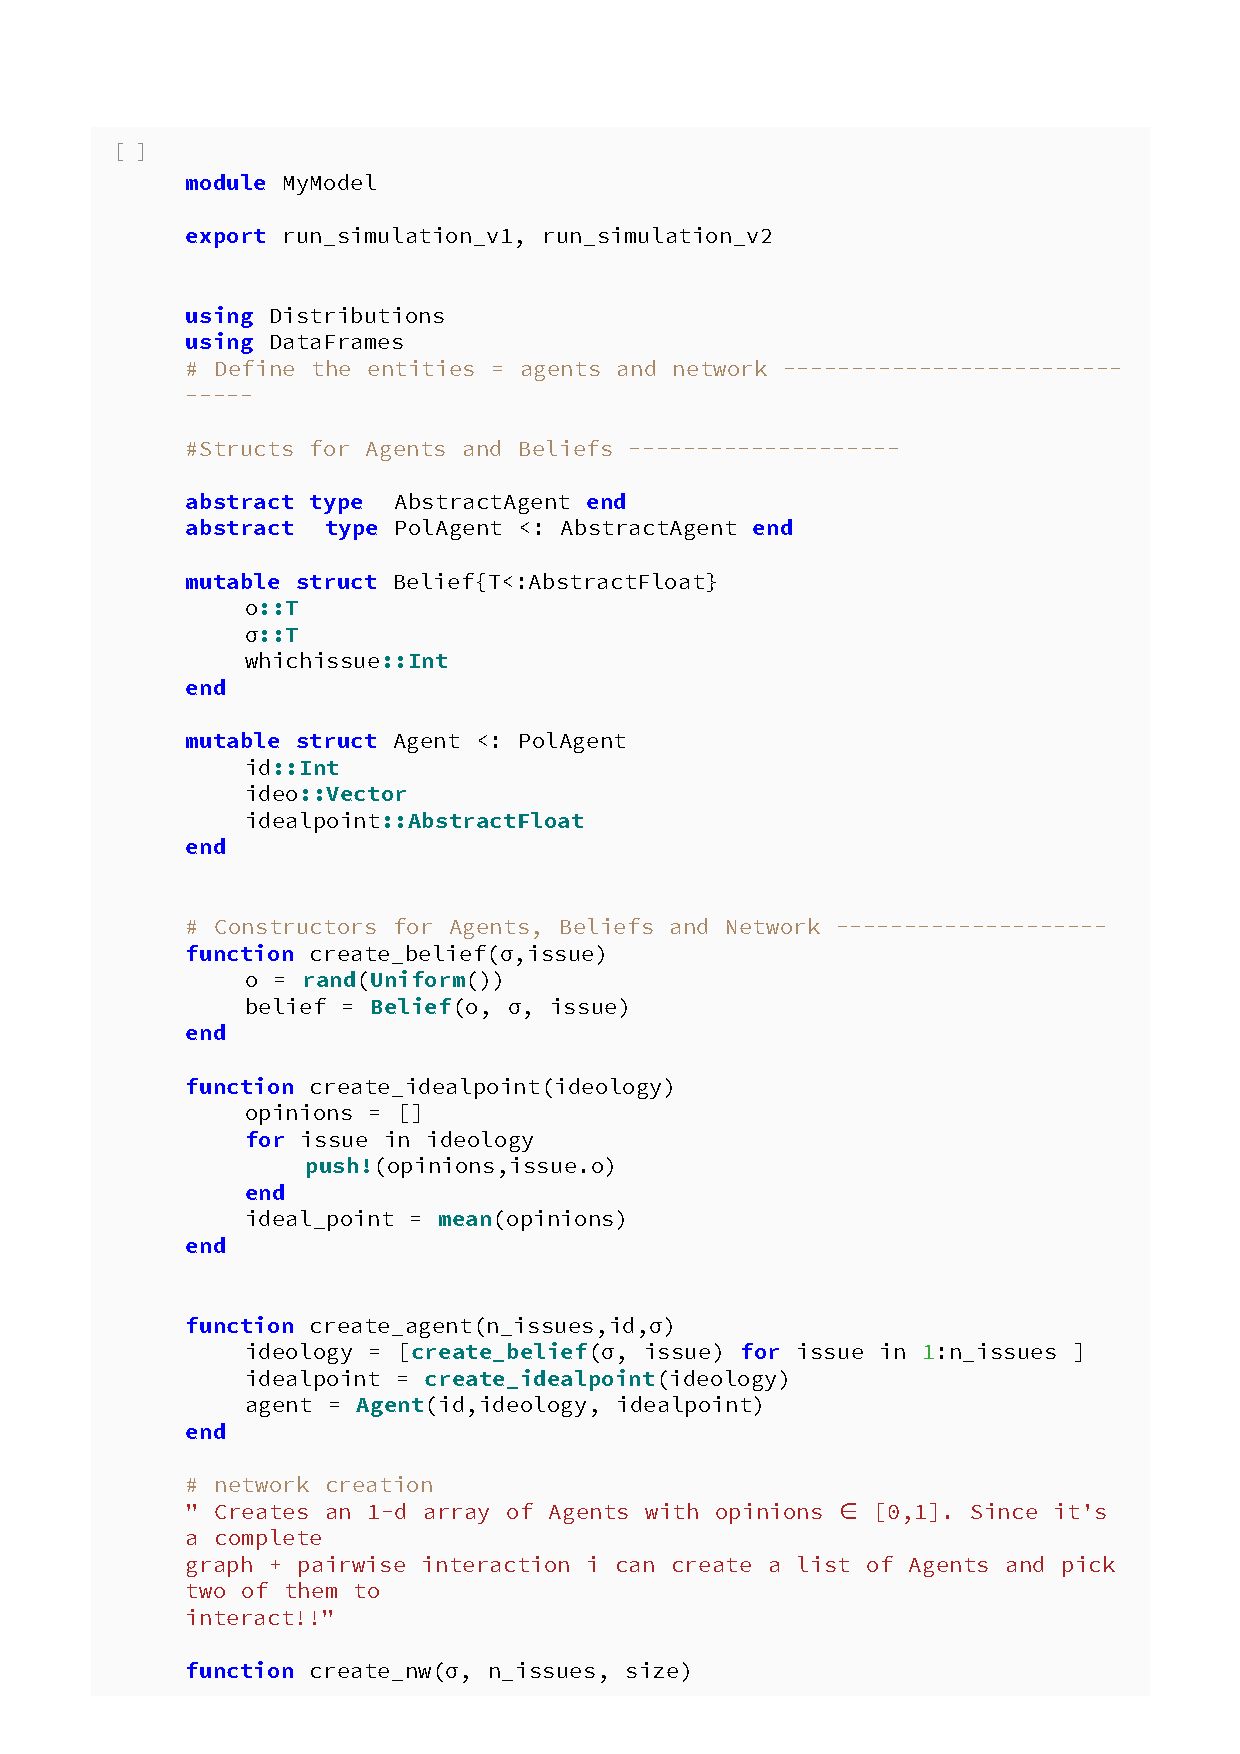
\includepdf[pages = {1,2,3,4}, pagecommand = {}, scale = 0.9]{ims/mymodel.pdf}
